%%%%%%%%%%%%%%%%%%%%%%%%%%%%%%%%%%%%%%%%%%%%%%%%%%%%%%%%%%%%%%%%%%%%%%%%%%%%%%%%
%2345678901234567890123456789012345678901234567890123456789012345678901234567890
%        1         2         3         4         5         6         7         8

\documentclass[letterpaper, 10 pt, conference]{ieeeconf}  % Comment this line out
                                                          % if you need a4paper
%\documentclass[a4paper, 10pt, conference]{ieeeconf}      % Use this line for a4
                                                          % paper

\IEEEoverridecommandlockouts                              % This command is only
                                                          % needed if you want to
                                                          % use the \thanks command
\overrideIEEEmargins
% See the \addtolength command later in the file to balance the column lengths
% on the last page of the document



% The following packages can be found on http:\\www.ctan.org
%\usepackage{graphics} % for pdf, bitmapped graphics files
%\usepackage{epsfig} % for postscript graphics files
%\usepackage{mathptmx} % assumes new font selection scheme installed
%\usepackage{times} % assumes new font selection scheme installed
%\usepackage{amsmath} % assumes amsmath package installed
%\usepackage{amssymb}  % assumes amsmath package installed
\usepackage{standalone} % for including tikz documents
\usepackage{tikz}
\usepackage{listings}
\usepackage{verbatim} % for multi line comments

\title{\LARGE \bf
Automated Three Vessel Home Brewing System*
}

%\author{ \parbox{3 in}{\centering Huibert Kwakernaak*
%         \thanks{*Use the $\backslash$thanks command to put information here}\\
%         Faculty of Electrical Engineering, Mathematics and Computer Science\\
%         University of Twente\\
%         7500 AE Enschede, The Netherlands\\
%         {\tt\small h.kwakernaak@autsubmit.com}}
%         \hspace*{ 0.5 in}
%         \parbox{3 in}{ \centering Pradeep Misra**
%         \thanks{**The footnote marks may be inserted manually}\\
%        Department of Electrical Engineering \\
%         Wright State University\\
%         Dayton, OH 45435, USA\\
%         {\tt\small pmisra@cs.wright.edu}}
%}

\author{Alvin Thai$^{1}$ and Nicholas Pelham$^{2}$ \\
	Department of Computer Science and Engineering \\
    University of California - Riverside \\
    \tt\small athai005@ucr.edu npelh001@ucr.edu
\thanks{*The system is simulated. No alcoholic beverages were made during the course of this project, but some were consumed.}% <-this % stops a space
\thanks{$^{1}$A. Thai is a Senior Computer Engineering Major who is too young to have as yet enjoyed a good beer}%
\thanks{$^{2}$N. Pelham is a Senior Computer Engineering Major with a decade of experience in and around the San Diego craft beer industry}%
}


\begin{document}



\maketitle
\thispagestyle{empty}
\pagestyle{empty}


%%%%%%%%%%%%%%%%%%%%%%%%%%%%%%%%%%%%%%%%%%%%%%%%%%%%%%%%%%%%%%%%%%%%%%%%%%%%%%%%
\begin{abstract}

Brewing beer at home is a popular hobby of craft beer enthusiasts. In this paper, we layout the requirements and designs for our proposed system to automate the process of creating wort, the sugary liquid extract which is fermented into beer. The fermentation process is not considered here, as it involves storing the wort and yeast mixture for several weeks until fermentation is complete. 

Automating the home brewing process reduces the risk of infection, improving the quality of the finished brew; and reduces the barrier to entry caused by the complexities in the process, allowing people to more easily enter the home brewing markets.

\end{abstract}


%%%%%%%%%%%%%%%%%%%%%%%%%%%%%%%%%%%%%%%%%%%%%%%%%%%%%%%%%%%%%%%%%%%%%%%%%%%%%%%%
\section{INTRODUCTION}

The majority of small batch home brewing is accomplished using recipe kits containing malt extract, which greatly limits the brewers' available creative options. The alternative method, all grain brewing, allows for greater opportunities to create unique brews. The process requires two additional vessels, additional ingredients, a noticeable amount of additional work.

Malt extract brewing is accomplished with a single vessel. Water is brought to a boil for a certain amount of time, and ingredients are added at various specified times within the boil at the end of which the wort is chilled either by allowing the mixture to sit until it's temperature falls to a specified temperature, by submerging the vessel in an ice bath, or by use of an immersion chiller.

In contrast, all grain brewing is accomplished most frequently with three vessels. Water is brought to a desired temperature within the first vessel, referred to as the Hot Liquor Tank. The Hot Liquor Tank's purpose is to bring water to a required temperature to be added to the Mash Tun, the second vessel. The Mash Tun is where the process of extracting malt sugars from grains is done by allowing the grains to soak within heated water until the starch within the grain is converted naturally to sugars. The water, now high in sugar content, is then moved into the final vessel in the process: the Boil Kettle. The Boil Kettle is in effect the single vessel used in malt extract brewing, and the process is similar with the difference of not requiring malt extract, syrups, or sugars to be added.

\section{MECHANICAL SYSTEM DESIGN}

The goal of our mechanical system design is to reduce the cost of the final product by utilizing parts within the system to accomplish multiple tasks. To this effect, we have chosen a single pump design which uses solenoid valves to direct the flow of liquid between all three vessels. A single heat exchange coil is used both for a heat exchange recirculating mash system (HERMS), and as an immersion chiller to crash cool the finished wort. The drawback of the system is that a single pump limits the systems ability to continuously sparge the mash, forcing a psuedo fly sparge to be implemented instead.

\begin{figure}[!htb]
  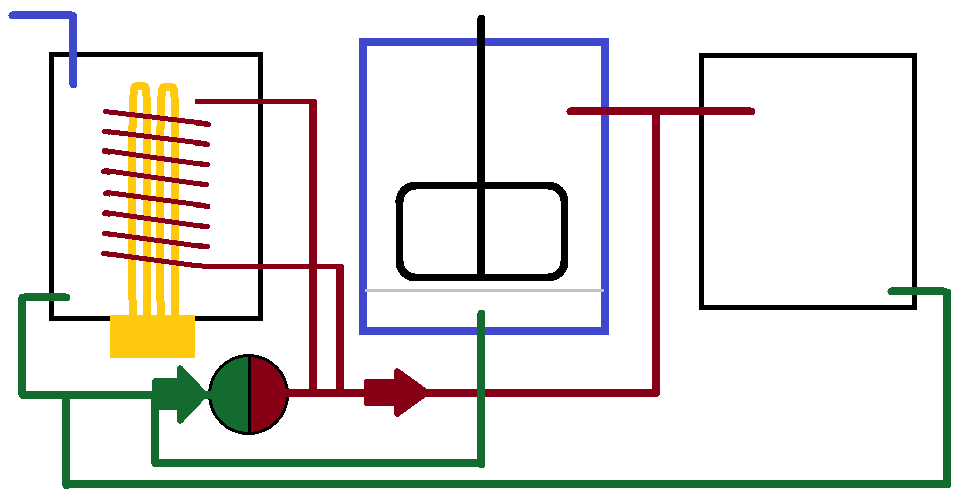
\includegraphics[width=0.5\textwidth]{3vbs}
  \caption{Mechanical System Design}
  \label{mec:diagram}
  % TODO: Labels on the diagram
\end{figure}

Liquid moves primarily from from the Hot Liquor Tank through the Mash Tun to the Boil Kettle (left to right in Fig. \ref{mec:diagram}). The Hot Liquor Tank must be filled with liquid at all stages of the process to facilitate the HERMS design of the Mash Tun and the crash cool operation of the Boil Kettle. The implication of these design choices is that each stage maintains some activity from it's first activation to the end of the brewing process.

\section{STATE MACHINE DESIGN}

\subsection{Hot Liquor Tank} 

\begin{figure}[!htb]
  \centering
  \includestandalone[mode=buildnew, width=0.5\textwidth]{HLT_SM}
  \caption{Hot Liquor Tank State Machine}
  \label{sm:hlt}
\end{figure}

In the initial stage of brewing, the HLT is filled with water and heats it up to a desired temperature. It remains in the \texttt{BelowTemp} state so long as the current temperature is lower than the desired temperature, then immediately finishes once the desired temperature is reached. The water is then transferred to the Mash Tun for the HERMS stage. 

During the mash, the HLT is required by the HERMS design to keep its volume of water at a specific temperature for a prolonged period of time. This is achieved with a \texttt{Persist} flag, which tells the HLT not to immediately finish after the water is heated to the desired temperature. When this flag is set, the heater is turned on when the current temperature is lower than the desired temperature, and off when the desired temperature is reached. At the end of the mash, all hot water is transferred to the Mash Tun to make room for cold water for the crash cool operation.

During the crash cool operation of the Boil Kettle, the desired temperature is set low such that the heater does not turn on - effectively keeping the water at a low temperature.

\subsection{Mash Tun}

The purpose of the Mash Tun is to extract sugars from malted grains through a process called mashing. Mashing involves soaking crushed grains in hot water, activating enzymes to produce maltose. The resulting liquid is called wort (pronounced \textit{wert}) and is the foundation of what will become beer.

\begin{figure}[!htb]
  \centering
  \includestandalone[mode=buildnew, width=0.5\textwidth]{MT_SM}
  \caption{Mash Tun State Machine}
  \label{sm:mt}
\end{figure}

The state machine design of the Mash Tun (Fig. \ref{sm:mt}) is very similar to the Hot Liquor Tank (Fig. \ref{sm:hlt}). The system waits in an inactive state for the \texttt{mashTime} and the \texttt{desiredTemp} to be set. The Mash Tun then waits in an active state as the hot water is moved from the Hot Liquor Tank to the Mash Tun. The system transitions into alternating heating states after float sensors report that the vessel is full.

The Mash Tun makes use of a Heat Exchange Recirculating Mash System (HERMS) to maintain a suitable mash temperature. The HERMS reduces the need for precisely controlling heaters using PID controllers by removing the mash from the direct heating system. The removes the danger of burning the malt and allows for additional flexibility in temperature control.

\subsection{Boil Kettle}

The Boil Kettle is where the additional flavors are extracted from ingredients like hops. The ingredients are added in timed stages during the boil. The number and duration of stages is dependent on the recipe being brewed, and so cannot be directly designed for. 

\begin{figure}[!htb]
  \centering
  \includestandalone[mode=buildnew, width=0.5\textwidth]{BK_SM}
  \caption{Boil Kettle State Machine}
  \label{sm:bk}
\end{figure}

The Boil Kettle state machine design (Fig. \ref{sm:bk}) is only sightly different from the state machines for the Hot Liquor Tank (Fig. \ref{sm:hlt}) and the Mash Tun (Fig. \ref{sm:mt}). An additional state is added for rapidly cooling the boil to a temperature suitable for adding yeast. The addition of the yeast is outside of the designed system, as fermentation requires long term storage and no system interaction.

The Boil Kettle waits in an inactive state for the \texttt{boilTime} and the \texttt{desiredTemp} to be set. The system then waits in an active fill state as the wort is transferred from the Mash Tun. If the Mash Tun is emptied before the Boil Kettle is full, additional water is added from the Hot Liquor Tank.

The system then moves to alternating heating states which control a direct heating element in the system. Precise temperature control is not deemed necessary, as the importance of the boil is primarily to boil, and not to maintain specific temperatures lower than that of a boil. To separate stages of the boil used for adding additional ingredients, the Cool state is effectively skipped by not updating \texttt{desiredTemp} to a lower temperature specific to that state. This allows the Boil Kettle to cycle through it's entire design for each stage of the boil.

The \texttt{desiredTemp} of the Cool state will be set to an appropriately low temperature during the final stage of the boil. In this active context, the Cool state is used to crash cool the wort to a desired temperate. This is done by re-purposing the heat exchange coil used in the HERMS. In the Cool state, the Hot Liquor Tank is filled with cold water and the hot water from the boil is pumped through the heat exchange coil. This use of the heat exchange coil effectively cools down the temperature of the water faster than it would by simply waiting for the heat to dissipate through the air.

\subsection{Control System}

The transportation of the liquid between all three vessels is done by a separate state machine being run on a distinct microcontroller. Because the flow of the liquid is not entirely linear, and several vessels are active at once, the state machine is designed for the majority of states to be accessible from an active waiting state.

\begin{figure}[!htb]
  \centering
  \includestandalone[mode=buildnew, width=0.5\textwidth]{Valves_SM}
  \caption{Pump Control State Machine}
  \label{sm:valves}
\end{figure}

The Pump Control state machine design (Fig. \ref{sm:valves}) makes the purpose for the previous state machine's uniformity more clear. By maintaining identical states in the various vessel designs, the Pump Control system can use knowledge of the states which those vessels are in to direct it's own transitions.

The single pump design of the physical system limits our design to a single transportation process at a time. This restricts our systems ability of execute a continuous (or fly) sparge to wash the grain from the Mash Tun. A continuous sparge is done by draining the Mash Tun into the Boil Kettle while simultaneously draining hot water from the Hot Liquor Tank to the Mash Tun.

While the system is designed to be flexible for different brewing recipes and styles, this is one limitation that is difficult to get around. A pseudo continuous sparge can be done by alternating between MTtoBK and HLTtoMT with minor changes to the design to allow it to skip the LeadMT state.

The LeadMT state is a short process that directly follows the Mash. Small particles of grain fall through the false bottom of the Mash Tun during the mash and need to be cycled back into the Mash Tun before the wort can be pumped into the Boil Kettle. This is done to avoid off flavors that can be caused by inadvertently boiling some of the malt.

\section{SPI PROTOCOLS}

All SPI communication is done by passing a \texttt{struct SPI\_Data} (detailed in Fig. \ref{spi:struct}) filled with both useful data, and null data used to conform to a single communication standard between all functions. A circular buffer is used to transmit the structure one byte at a time, and a function is called when the final byte is received. The function \texttt{void handleReceivedData(void)} is defined for each component to handle receiving the data differently.

\begin{figure}[thpb]
\begin{center}
\begin{tabular}{|c|}
\hline
\begin{lstlisting}
struct SPI_Data {
    unsigned char  flag;
    unsigned short temp;
    signed   short time;
    unsigned char  vol;
}
\end{lstlisting} \\
\hline
\end{tabular}
\end{center}
\caption{Data type used for SPI communication}
\label{spi:struct}
\end{figure}

Slave systems have a slight variation on \texttt{struct SPI\_Data} which contains an unused member of type char which is used to allow the transfer a single additional transmission byte for the slave to finish sending data to the master. The master sends a byte of \texttt{0x00} to fill this unused member.

The \texttt{Flag} member variable is set to \texttt{0xFF} by the master to instruct the slave to ignore all incoming data. This allows the master to poll slaves for data required for it's operation without interfering with their current state by sending data which may have been changed by the slaves systems.

\section{COMPLEXITIES}

The complexity involved in our design comes largely from utilizing multiple ATMega1284 controllers, a requirement for the Intermediate Embedded Systems course which this system is designed within. A single ATMega is used to control each individual vessel, each connected through SPI to a single master which controls the transportation mechanisms and acts as an interface through which a user operates the system. The synchronization of all of these tasks is expected to fulfill most of the assignment's complexity requirements.

Hardware complexities include thermal resistors used to monitor the temperature within each vessel, liquid flow meters to monitor the amount of liquid entering the hot liquor tank and the boil kettle, and float switches to monitor the level of the mash tun. Additionally, and time permitting, an LCD touchscreen will be implemented on the master controller as a user interface through which all processes will be controlled, and all variables will be displayed.

\section{LIMITATIONS}

Because of limited time, funding being provided exclusively by ourselves, and the focus of the course for which this product is being developed; several key components will not be included in the product presented at the end of the course. These include all physical vessels, pipes, valves, heaters, and the pump. Valves and heaters will be simulated using LEDs, the pump will be simulated using a DC motor, and the stirring motor for the mash tun will be simulated with a smaller stepper motor.

The initial prototype used for testing will make use of several available parts which function similar to the parts expected to be included in the graded project. In the event that the parts are not delivered in a timely manner, the simulated parts will be used in the presentation. These parts include: potentiometers in place of thermal resistors, mechanical switches in place of float switches, and software timers in place of flow sensors.

\section{PROBLEMS}

The presented product is not automated from start to finish. The method used to poll systems for data using SPI introduced garbage data that circulated through the systems. The garbage data interfered with automation processes that relied heavily on constant polling of the slaves by the master. Without this data, the automation processes were unable to function as designed.

\section{PRODUCT PRESENTATION}

The final presentation for the course will be done using primarily simulated parts. A drawing, or other mock up available at the time of the presentation, will be displayed with LEDs, a stepper motor, and a DC motor in appropriately visible locations so as to demonstrate the desired functionality of the product. Timers will be set to appropriately short intervals so as to complete the demonstration in a timely manner.

\section{CONCLUSIONS}

The complexity of the system as required for the course for which it was designed proved to be detrimental to the final product. Not only does it require additional expense through unnecessary parts, but the complications introduced by creating a network of interdependent systems is difficult to implement.

A better solution would be to integrate all three vessels and the pump control system into a single controller. The cost of the unit, as it pertains to the embedded system, would be greatly reduced by removing the duplicate controllers. The close proximity of the three systems also makes physical separation of their controls unnecessary.

\addtolength{\textheight}{-12cm}   % This command serves to balance the column lengths
                                  % on the last page of the document manually. It shortens
                                  % the textheight of the last page by a suitable amount.
                                  % This command does not take effect until the next page
                                  % so it should come on the page before the last. Make
                                  % sure that you do not shorten the textheight too much.

%%%%%%%%%%%%%%%%%%%%%%%%%%%%%%%%%%%%%%%%%%%%%%%%%%%%%%%%%%%%%%%%%%%%%%%%%%%%%%%%



%%%%%%%%%%%%%%%%%%%%%%%%%%%%%%%%%%%%%%%%%%%%%%%%%%%%%%%%%%%%%%%%%%%%%%%%%%%%%%%%



%%%%%%%%%%%%%%%%%%%%%%%%%%%%%%%%%%%%%%%%%%%%%%%%%%%%%%%%%%%%%%%%%%%%%%%%%%%%%%%%
\begin{comment}
\section*{APPENDIX}

Appendixes should appear before the acknowledgment.

\end{comment}

\section*{ACKNOWLEDGMENT}

The real-time operating system used for this product is a version of FreeRTOS provided by UCR for the Intermediate Embedded Systems course.


%%%%%%%%%%%%%%%%%%%%%%%%%%%%%%%%%%%%%%%%%%%%%%%%%%%%%%%%%%%%%%%%%%%%%%%%%%%%%%%%

\begin{comment}
References are important to the reader; therefore, each citation must be complete and correct. If at all possible, references should be commonly available publications.



\begin{thebibliography}{99}

\bibitem{c1} G. O. Young, ÒSynthetic structure of industrial plastics (Book style with paper title and editor),Ó 	in Plastics, 2nd ed. vol. 3, J. Peters, Ed.  New York: McGraw-Hill, 1964, pp. 15Ð64.






\end{thebibliography}
\end{comment}



\end{document}
